\chapter{ターミナルに慣れる}
\sheet{4-1〜4-3}

この章では、Git Bash でフォルダやファイルを操作する練習をします。
エクスプローラーでマウスを使ってやっていることを、文字で命令するだけです。

\section{GUI と CLI}

\begin{center}\small
\begin{tabularx}{\linewidth}{l X X}
\toprule
 & GUI（グラフィカル） & CLI（コマンドライン） \\
\midrule
操作 & マウスでアイコンをクリック & 文字で命令を打つ \\
例 & エクスプローラー、Word & Git Bash、PowerShell \\
得意なこと & 見て分かる、迷わない & 繰り返し・正確さ・記録に残る・AI と相性がよい \\
\bottomrule
\end{tabularx}
\end{center}

開発で CLI を使う最大の理由は、\textbf{やったことが文字で残る}ことです。
「さっき何をしたっけ？」と聞かれたときに、打ったコマンドをそのまま見せれば済みます。
Claude Code が裏で実行しているのも、同じコマンドです。

\section{プロンプトの読み方}

\begin{wintermwin}[0.85\linewidth]{MINGW64:/c/Users/ryusei/dev}
{\color{matcha!70!white}ryusei@DESKTOP-AB12CD} {\color{violet!50!white}MINGW64} {\color{kincha!80!white}\textasciitilde/dev}\\
\$ \_
\end{wintermwin}

\begin{itemize}
  \item \code{ryusei@DESKTOP-AB12CD}：ユーザー名@PC の名前
  \item \code{\textasciitilde/dev}：\textbf{いま居る場所}（カレントディレクトリ）。\code{\textasciitilde} はホームフォルダ \verb|C:\Users\ryusei| のこと
  \item \code{\$}：ここに命令を打ってください、という印
\end{itemize}

\section{パス：ファイルの住所}

\term{パス}はファイルやフォルダの「住所」です。Git Bash では区切りに \code{/}（スラッシュ）を使います。

\begin{center}
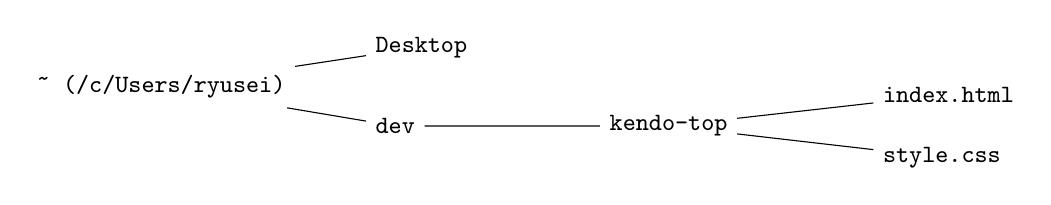
\begin{tikzpicture}[font=\ttfamily\small,grow'=right,level distance=2.6cm,
  level 1/.style={sibling distance=1cm},level 2/.style={sibling distance=0.8cm},
  every node/.style={anchor=west}]
\node {\textasciitilde\ (/c/Users/ryusei)}
  child {node {Desktop}}
  child {node {dev}
    child {node {kendo-top}
      child {node {index.html}}
      child {node {style.css}}}
  };
\end{tikzpicture}
\end{center}

\begin{itemize}
  \item \term{絶対パス}：一番上から書く住所。例：\code{/c/Users/ryusei/dev/kendo-top/index.html}
  \item \term{相対パス}：いま居る場所から見た住所。\code{dev} に居るなら \code{kendo-top/index.html}
  \item \code{.}（ドット1つ）は「いま居る場所」、\code{..}（ドット2つ）は「1つ上の階層」
\end{itemize}

\section{基本コマンド}

\begin{center}\small
\begin{tabularx}{\linewidth}{l l X}
\toprule
コマンド & 由来 & すること \\
\midrule
\code{pwd} & print working directory & いま居る場所を表示する \\
\code{ls} & list & 中にあるファイル・フォルダを一覧表示する（\code{ls -a} で隠しファイルも） \\
\code{cd 場所} & change directory & 移動する。\code{cd ..} で1つ上、\code{cd} だけでホームに戻る \\
\code{mkdir 名前} & make directory & フォルダを作る \\
\code{touch 名前} & & 空のファイルを作る \\
\code{cat ファイル} & concatenate & ファイルの中身を表示する \\
\code{cp 元 先} & copy & コピーする \\
\code{mv 元 先} & move & 移動する／名前を変える \\
\code{rm ファイル} & remove & 削除する（\textbf{ゴミ箱に入らない}） \\
\code{code .} & & いまの場所を VS Code で開く \\
\code{explorer .} & & いまの場所をエクスプローラーで開く \\
\code{clear} & & 画面をきれいにする（\key{Ctrl}+\key{L} でも同じ） \\
\bottomrule
\end{tabularx}
\end{center}

\begin{caution}[rm は取り消せない]
\code{rm} で消したファイルはゴミ箱に入らず、そのまま消えます。
特に \code{rm -rf}（フォルダごと強制削除）は、場所を間違えると大事なものまで消えます。
Claude Code が \code{rm -rf} を実行しようとしたら、\textbf{どこを消そうとしているのか必ず確かめてから}許可してください。
\end{caution}

\section{便利な操作}

\begin{center}\small
\begin{tabularx}{\linewidth}{l X}
\toprule
操作 & 効果 \\
\midrule
\key{Tab} & 名前の続きを自動で補完する。\textbf{打ち間違いが減るので積極的に使う} \\
\key{↑} \key{↓} & 前に打ったコマンドを呼び出す \\
\key{Ctrl}+\key{C} & 実行中のコマンドを止める（Git Bash ではコピーではない） \\
\key{Shift}+\key{Insert} & 貼り付け（右クリック → Paste でも可） \\
\code{q} & \code{git log} などの一覧表示から抜ける \\
\bottomrule
\end{tabularx}
\end{center}

\section{ハンズオン}

\begin{step}{作業フォルダを作る}
\sheet{4-2}
\begin{terminal}[Git Bash]
$ cd
$ pwd
/c/Users/ryusei
$ mkdir dev
$ cd dev
$ pwd
/c/Users/ryusei/dev
\end{terminal}
これで、作業フォルダ \verb|~/dev| ができました。この先の作業は、すべてこの中で行います。
\end{step}

\begin{step}{練習用のフォルダとファイルを作って動かす}
\begin{terminal}[Git Bash]
$ mkdir terminal-practice
$ cd terminal-practice
$ touch memo.txt
$ echo "面打ち 100本" > memo.txt
$ cat memo.txt
面打ち 100本
$ echo "小手面 50本" >> memo.txt
$ cat memo.txt
面打ち 100本
小手面 50本
$ cp memo.txt memo-backup.txt
$ ls
memo-backup.txt  memo.txt
$ mv memo-backup.txt old.txt
$ ls
memo.txt  old.txt
$ rm old.txt
$ ls
memo.txt
\end{terminal}
\code{>} はファイルに上書き、\code{>>} はファイルの末尾に追記、という意味です。
\end{step}

\begin{step}{VS Code とエクスプローラーで確かめる}
\begin{terminal}[Git Bash]
$ code .
$ explorer .
\end{terminal}
VS Code とエクスプローラーの両方で \code{memo.txt} が見えれば、
「ターミナルで操作したものと、マウスで見ているものは同じもの」だと確かめられたことになります。
\end{step}

\begin{challenge}{ターミナルだけで部の稽古メモを作る}
\sheet{4-3}
マウスを使わずに、次の状態を作ってください。
\begin{enumerate}
  \item \verb|~/dev/terminal-practice| の中に \code{keiko} というフォルダを作る
  \item その中に \code{monday.txt} と \code{thursday.txt} を作り、それぞれに稽古メニューを2行ずつ書く
  \item \code{thursday.txt} を \code{saturday.txt} という名前に変える
  \item \code{cat} で2つのファイルの中身を表示し、その画面をスクショしてスプシの詰まりメモ欄に「完了」と書く
\end{enumerate}
\end{challenge}

\begin{checklist}
\begin{itemize}
  \checkitem プロンプトを見て、いま居る場所を言える
  \checkitem 絶対パスと相対パスの違いを説明できる
  \checkitem \code{cd}・\code{ls}・\code{mkdir}・\code{cat} を、表を見ずに使える
  \checkitem \key{Tab} で補完できる
  \checkitem \code{rm} が危ない理由を言える
\end{itemize}
\end{checklist}
